%Dokumentinformationen
\newcommand{\titleinfo}{ProGru - Zusammenfassung}
\newcommand{\authorinfo}{L. Leuenberger}
\newcommand{\versioninfo}{$Revision: $ \today}

% standard header
%Schriftgr�sse, Layout, Papierformat, Art des Dokumentes
\documentclass[10pt,twoside,a4paper,fleqn]{article}
%Einstellungen der Seitenr�nder
\usepackage[left=1cm,right=1cm,top=1cm,bottom=1cm,includeheadfoot]{geometry}
% Sprache, Zeichensatz, packages
\usepackage[ansinew]{inputenc}
\usepackage[ngerman]{babel,varioref}
\usepackage{amssymb,amsmath,fancybox,graphicx,color,lastpage,wrapfig,fancyhdr,hyperref,verbatim}

%pdf info
\hypersetup{pdfauthor={\authorinfo},pdftitle={\titleinfo},colorlinks=false}
%linkbordercolor=white
\author{\authorinfo}
\title{\titleinfo}

%Kopf- und Fusszeile
\pagestyle{fancy}
\fancyhf{}
%Linien oben und unten
\renewcommand{\headrulewidth}{0.5pt} 
\renewcommand{\footrulewidth}{0.5pt}

\fancyhead[L]{\titleinfo{ }\tiny{(\versioninfo)}}
%Kopfzeile rechts bzw. aussen
\fancyhead[R]{Seite \thepage { }von \pageref{LastPage}}
%Fusszeile links bzw. innen
\fancyfoot[L]{\footnotesize{\authorinfo}}
%Fusszeile rechts bzw. ausen
\fancyfoot[R]{\footnotesize{\today}} % ./header.tex nicht editieren (Projekt LaTeX-Header benutzen)

%%%%%%%%%%%%%%%%%%%%%%%%%%%%%%%%%%%%%%%%%%%%%%%%%%%%%%%%%%%%%%%%%%%%%%%%%%%%%%%%%%%%%%%%%%%%%%%%
% Neue Befehle und Definitionen                
%%%%%%%%%%%%%%%%%%%%%%%%%%%%%%%%%%%%%%%%%%%%%%%%%%%%%%%%%%%%%%%%%%%%%%%%%%%%%%%%%%%%%%%%%%%%%%%
% This is needed for one more subsection, ex. 1.1.1.1, is called by \paragraph{}
\usepackage{titlesec}
\setcounter{secnumdepth}{4}
\setcounter{tocdepth}{4}
\titleformat{\paragraph}
{\normalfont\normalsize\bfseries}{\theparagraph}{1em}{}
% Settings which are used to set the distance above and under the sections
\titlespacing*{\paragraph}{0pt}{2.25ex plus 1ex minus .2ex}{1.0ex plus .2ex}
\titlespacing{\section}{0em}{0.5em}{0.5em}
\titlespacing{\subsection}{0em}{0.5em}{0.5em}
\titlespacing{\subsubsection}{0em}{0.5em}{0.5em}

% Linksb�ndig
\setlength\parindent{0ex}

% This is needed for a smaller itemlist, is called by \compactenum {}
\usepackage{paralist}

% This is needed for merging some columns in a table
\usepackage{multicol} 
\usepackage{multirow}

% This is needed for code listing
\usepackage{listings}

\definecolor{red}{rgb}{1,0,0}
\newcommand{\verweis}[1]{$_{\textcolor{red}{\mbox{\small{Kapitel #1}}}}$}

%Document Anfang
\begin{document}	
\section{Vom Problem zum Programm \verweis{1.2}}
	\subsection{Algorithmus}
		Der Begriff Programm ist eng mit dem Begriff Algorithmus verbunden. Algorithmen sind Vorschriften f�r die L�sung eines Problemes, welches die Handlungen und ihre Abfolge, also die Handlungsweise, beschreiben. Abstrakt kann man sagen, dass die folgenden Bestandteile und Eigenschaften zu einem Algorithmus geh�ren: \textit{(am Beispiel eines Kochrezeptes erkl�rt)} 
		\begin{compactitem}
			\item eine \textbf{Menge von Objekten}, die durch den Algorithmus bearbeitet werden \textit{(Zutaten, Geschirr, Herd, \dots)}
			\item eine \textbf{Menge von Operationen}, die auf den Objekten ausgef�hrt werden \textit{(waschen, sch�len, \dots)}
			\item ein \textbf{definierter Anfangszustand}, in dem sich die Objekte zu Beginn befinden \textit{(Teller leer, Herd kalt, \dots)}
			\item ein \textbf{gew�nschter Endzustand}, in dem sich die Objekte nach der L�sung des Problems befinden sollen \textit{(gekochtes Gem�se, \dots)}
		\end{compactitem}	

	\subsection{Der euklidische Algorithmus als Beispiel}
		\subsubsection{Das Problem}
				Eine rechteckige Terrasse sei mit m�glichst grossen quadratischen Platten auszulegen. Welche Kantenl�nge haben die Platten?
			
		\begin{minipage}[t]{9 cm}
			\subsubsection{Der Algorithmus}
				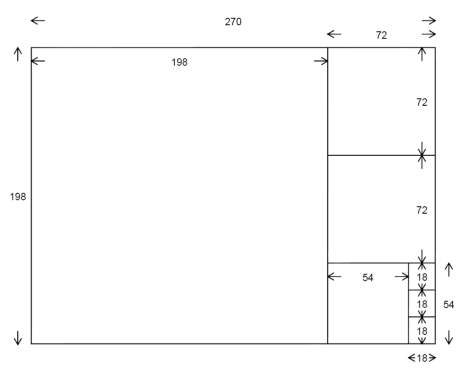
\includegraphics[width=1.0\textwidth]{pics/Euklid.jpg}
							
				Mit Abschneidetechnik nach Euklid. Entspricht der \\
				Ermittlung des gr�ssten gemeinsamen Teilers (ggT): \\
				$\frac{x_{ungek"urzt}}{y_{ungek"urzt}}=\frac{\frac{x_{ungek"urzt}}{ggT(x_{ungek"urzt},y_{ungek"urzt})}}{\frac{y_{ungek"urzt}}{ggT(x_{ungek"urzt},y_{ungek"urzt})}}=\frac{x_{gek"urzt}}{y_{gek"urzt}}$ \\
					
			\subsubsection{Algorithmus-Beschreibung mit Struktogramm \verweis{1.3}}
				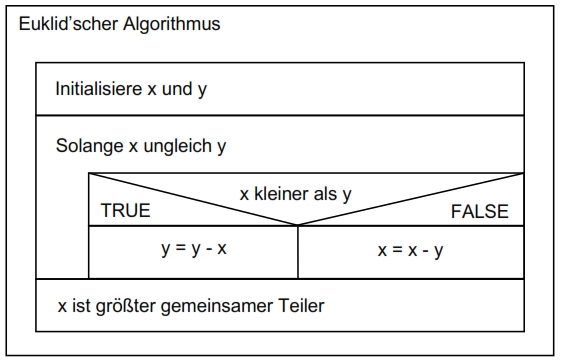
\includegraphics[width=1.0\textwidth]{pics/Euklid_Struktogramm.jpg}

		\end{minipage}
		%
		\begin{minipage}[t]{9 cm}	
			\subsubsection{Algorithmus-Beschreibung mit Pseudocode \verweis{1.2.1}}
				\lstinputlisting[language=C,tabsize=2]{code/Euklid_Pseudo.c}
					
				\subsubsection{Programm}
					\lstinputlisting[language=C,tabsize=2]{code/Euklid.c}
							
				\subsubsection{Trace-Tabelle \verweis{1.2.4}}
					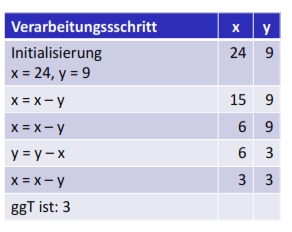
\includegraphics[width=0.58\textwidth]{pics/Euklid_Trace.jpg}
	
		\end{minipage}
		
\newpage
		
	\subsection{Nassi-Shneiderman-Diagramme \verweis{1.3}}
		Zur Visualisierung des Kontrollflusses von Programmen, das heisst, zur grafischen Veranschaulichung ihres Ablaufes, wurden 1973 von Nassi und Shneiderman grafische Strukturen, die sogenannten Struktogramme, vorgeschlagen. Entwirft man Programme mit Nassi-Shneiderman-Diagrammen, so gen�gt man automatisch den Regeln der Strukturierten Programmierung.
		
		\begin{minipage}[t]{6 cm}
			\subsubsection{Sequenz}
				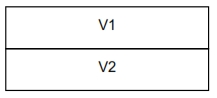
\includegraphics[width=1\textwidth]{pics/Nassi_Sequenz.jpg}
				
			\subsubsection{Block}
				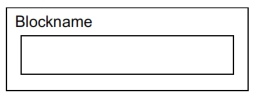
\includegraphics[width=1\textwidth]{pics/Nassi_Block.jpg}	
					
			\subsubsection{Einfache Alternative}
				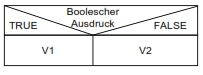
\includegraphics[width=1\textwidth]{pics/Nassi_einfache_Alternative.jpg}
					
		\end{minipage}
		%
		\begin{minipage}[t]{6 cm}
			\subsubsection{Bedingte Anweisung}
				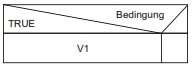
\includegraphics[width=1\textwidth]{pics/Nassi_bedingte_Verarbeitung.jpg}
								
			\subsubsection{Mehrfache Alternative}
				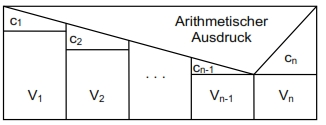
\includegraphics[width=1\textwidth]{pics/Nassi_mehrfache_Alternative.jpg}	
									
			\subsubsection{Schleife mit vorheriger Pr�fung}
				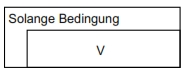
\includegraphics[width=1\textwidth]{pics/Nassi_While.jpg}
					
		\end{minipage}
		%
		\begin{minipage}[t]{6 cm}
			\subsubsection{Endlosschlaufe}
				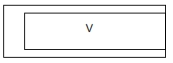
\includegraphics[width=1\textwidth]{pics/Nassi_While1.jpg}
											
			\subsubsection{Schleife mit nachfolgender Pr�fung}
				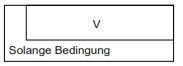
\includegraphics[width=1\textwidth]{pics/Nassi_DoWhile.jpg}	
					
			\subsubsection{Abbruchanweisung}
				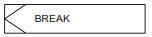
\includegraphics[width=1\textwidth]{pics/Nassi_Break.jpg}	
								
		\end{minipage}
		
\section{Kontrollstrukturen \verweis{8}}
	\begin{minipage}[t]{9 cm}
		\subsection{Sequenz \verweis{8.1}}
			Die Sequenz ist eine zeitlich geordnete Abfolge von Anweisungen. \\
				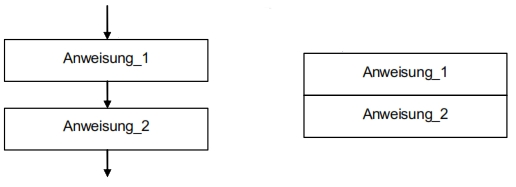
\includegraphics[width=1\textwidth]{pics/Sequenz.jpg}	
			
	\end{minipage}
	%
	\begin{minipage}[t]{9 cm}
			\subsubsection{Block}
				\begin{compactitem}
					\item Erfordert die Syntax genau eine Anweisung, so k�nnen dennoch mehrere Anweisungen geschrieben werden, wenn man sie in Form eines Blocks zusammenfasst.
					\item Ein Block wird mit geschweiften Klammern eingefasst. $\{ \dots \}$ Ein Block z�hlt syntaktisch als eine einzige Anweisung.
				\end{compactitem}
				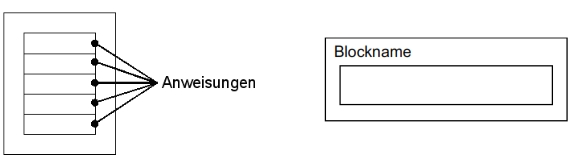
\includegraphics[width=1\textwidth]{pics/Block.jpg}
	\end{minipage}	
		
	\subsection{Selektion \verweis{8.2}}
		Von \textbf{Selektion} spricht man zum einen, wenn man eine Anweisung nur dann ausf�hren will, wenn eine bestimmte Bedingung zutrifft. Zum anderen m�chte man mit Selektionsanweisungen zwischen zwei M�glichkeiten (entweder/oder) bzw. zwischen mehreren M�glichkeiten genau eine ausw�hlen.
		
		\begin{minipage}[t]{5.5 cm}
			\subsubsection{Einfache Alternative}
				\lstinputlisting[language=C,tabsize=2]{code/strukturen_if_else.c}
		\end{minipage}
		%
		\begin{minipage}[t]{5.5 cm}
			\subsubsection{Bedingte Anweisung}
				\lstinputlisting[language=C,tabsize=2]{code/strukturen_if.c}
		\end{minipage}
		%
		\begin{minipage}[t]{7 cm}
			\subsubsection{Mehrfache Alternative - else if}
				\lstinputlisting[language=C,tabsize=2]{code/strukturen_else_if.c}
		\end{minipage}
		
\newpage

		\subsubsection{Mehrfache Alternative - switch case}
			\begin{minipage}[t]{9 cm}
				
				\begin{compactitem}
					\item F�r eine Mehrfach-Selektion, d.h. eine Selektion unter mehreren Alternativen, kann die $switch$-Anweisung verwendet werden, falls die Alternativen ganzzahligen Werten eines Ausdrucks von einem Integer-Typ entsprechen.
					\item Hat der Ausdruck der $switch$-Anweisung den gleichen Wert wie einer der konstanten Ausdr�cke der $case$-Marken, wird die Ausf�hrung des Programms mit der Anweisung hinter dieser $case$-Marke weitergef�hrt.
					\item Stimmt keiner der konstanten Ausdr�cke mit dem $switch$-Ausdruck �berein, wird zu $default$ gesprungen.
				\end{compactitem}							
			\end{minipage}
			\hspace*{1cm}
			\begin{minipage}[t]{9 cm}
				\vspace*{-0.5cm}
				\lstinputlisting[language=C,tabsize=2]{code/strukturen_switch.c}
			\end{minipage}
			
	\subsection{Iteration \verweis{8.3}}
		\begin{minipage}[t]{4 cm}
			\subsubsection{While}
				\lstinputlisting[language=C,tabsize=2]{code/strukturen_while.c}
		\end{minipage}
		%
		\begin{minipage}[t]{10 cm}
			\subsubsection{For-Schleife}
				\lstinputlisting[language=C,tabsize=2]{code/strukturen_for.c}
		\end{minipage}
		%
		\begin{minipage}[t]{5 cm}
			\subsubsection{Do-While}
				\lstinputlisting[language=C,tabsize=2]{code/strukturen_dowhile.c}
		\end{minipage}
		
		\subsubsection{Endlosschleife}
			\begin{minipage}[c]{3 cm}
				\lstinputlisting[language=C,tabsize=2]{code/strukturen_endlos_for.c}
			\end{minipage}
			%
			\begin{minipage}[c]{3 cm}
				\lstinputlisting[language=C,tabsize=2]{code/strukturen_endlos_while.c}
			\end{minipage}
		
		\subsubsection{Wann wird welche Schleife eingesetzt?}
			\begin{compactitem}
				\item For-Schleife: Bei Z�hlschleifen, d.h. wenn die Anzahl Durchl�ufe (kann auch variabel sein) im
				voraus feststeht.
				\item Do-While-Schleife: Wenn es keine Z�hlschleife ist, und die Schleife muss mindestens einmal
				durchlaufen werden
				\item While-Schleife: In allen anderen F�llen
			\end{compactitem}
			
	\subsection{Sprunganweisungen \verweis{8.4}}
		\begin{compactitem}
			\item break: $do-while$-, $while$-,  $for$-Schleife und $switch$-Anweisung abbrechen
			\item continue: in den n�chsten Schleifendurchgang (Schleifenkopf) springen bei $do-while$-, $while$- und $for$-Schleife 
			\item return: aus Funktion an aufrufende Stelle zur�ckspringen
			\item goto: innerhalb einer Funktion an eine Marke (Label) springen
		\end{compactitem}
		
\end{document}
